\subsection{Оптимизация модели}

Для оптимизации модели выбран фреймворк gsplat \cite{ye2024gsplatopensourcelibrarygaussian}. Параметры обучения выбраны стандартные. В качестве стратегии прунинга и уплотнения гауссиан были испробованы 2 стратегии: обычная (из оригинальной статьи) и упоминаемая ранее MCMC (Markov Chain Monte Carlo).

Чтобы выделить более удачную для текущей задачи стратегию, для оптимизации использовались все 700 кадров (это позволяет исключить проблемы нехватки данных). Из особенностей обучения, от стандартного 3DGS, можно выделить градиентный спуск не по всему прямоугольнику изображения, для этого каждой референсной картинке сопоставлена маска, отделяющая скелет от фона. Итоги обучения приведены на рисунке \ref{fig:default-vs-mcmc}.

\begin{figure}[htbp]
	\centering
	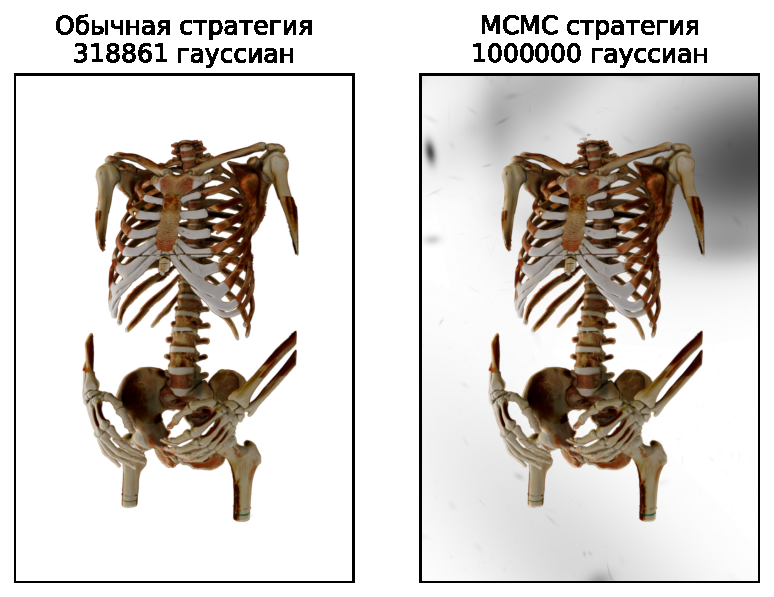
\includegraphics[width=0.7\textwidth]{assets/default-vs-mcmc.pdf}
	\caption{30000 итераций двух разных стратегий, где фоновым цветом выбран белый; стратегия MCMC выдаёт артефакты вокруг модели}
	\label{fig:default-vs-mcmc}
\end{figure}

Такой исход объясняется тем, что стратегия MCMC завязана на встряхивании гауссиан, поэтому они легко могут уйти на фон, на который оптимизация не смотрит.

На RTX 2060 6G обучение 30000 итераций занимает 15 минут времени.

Рисунок \ref{fig:50-100-250-700} демонстрирует различное количество референсных изображений для получения модели. По нему видно, что приемлемое качество достигается уже при 250.

\begin{figure}[htbp]
	\centering
	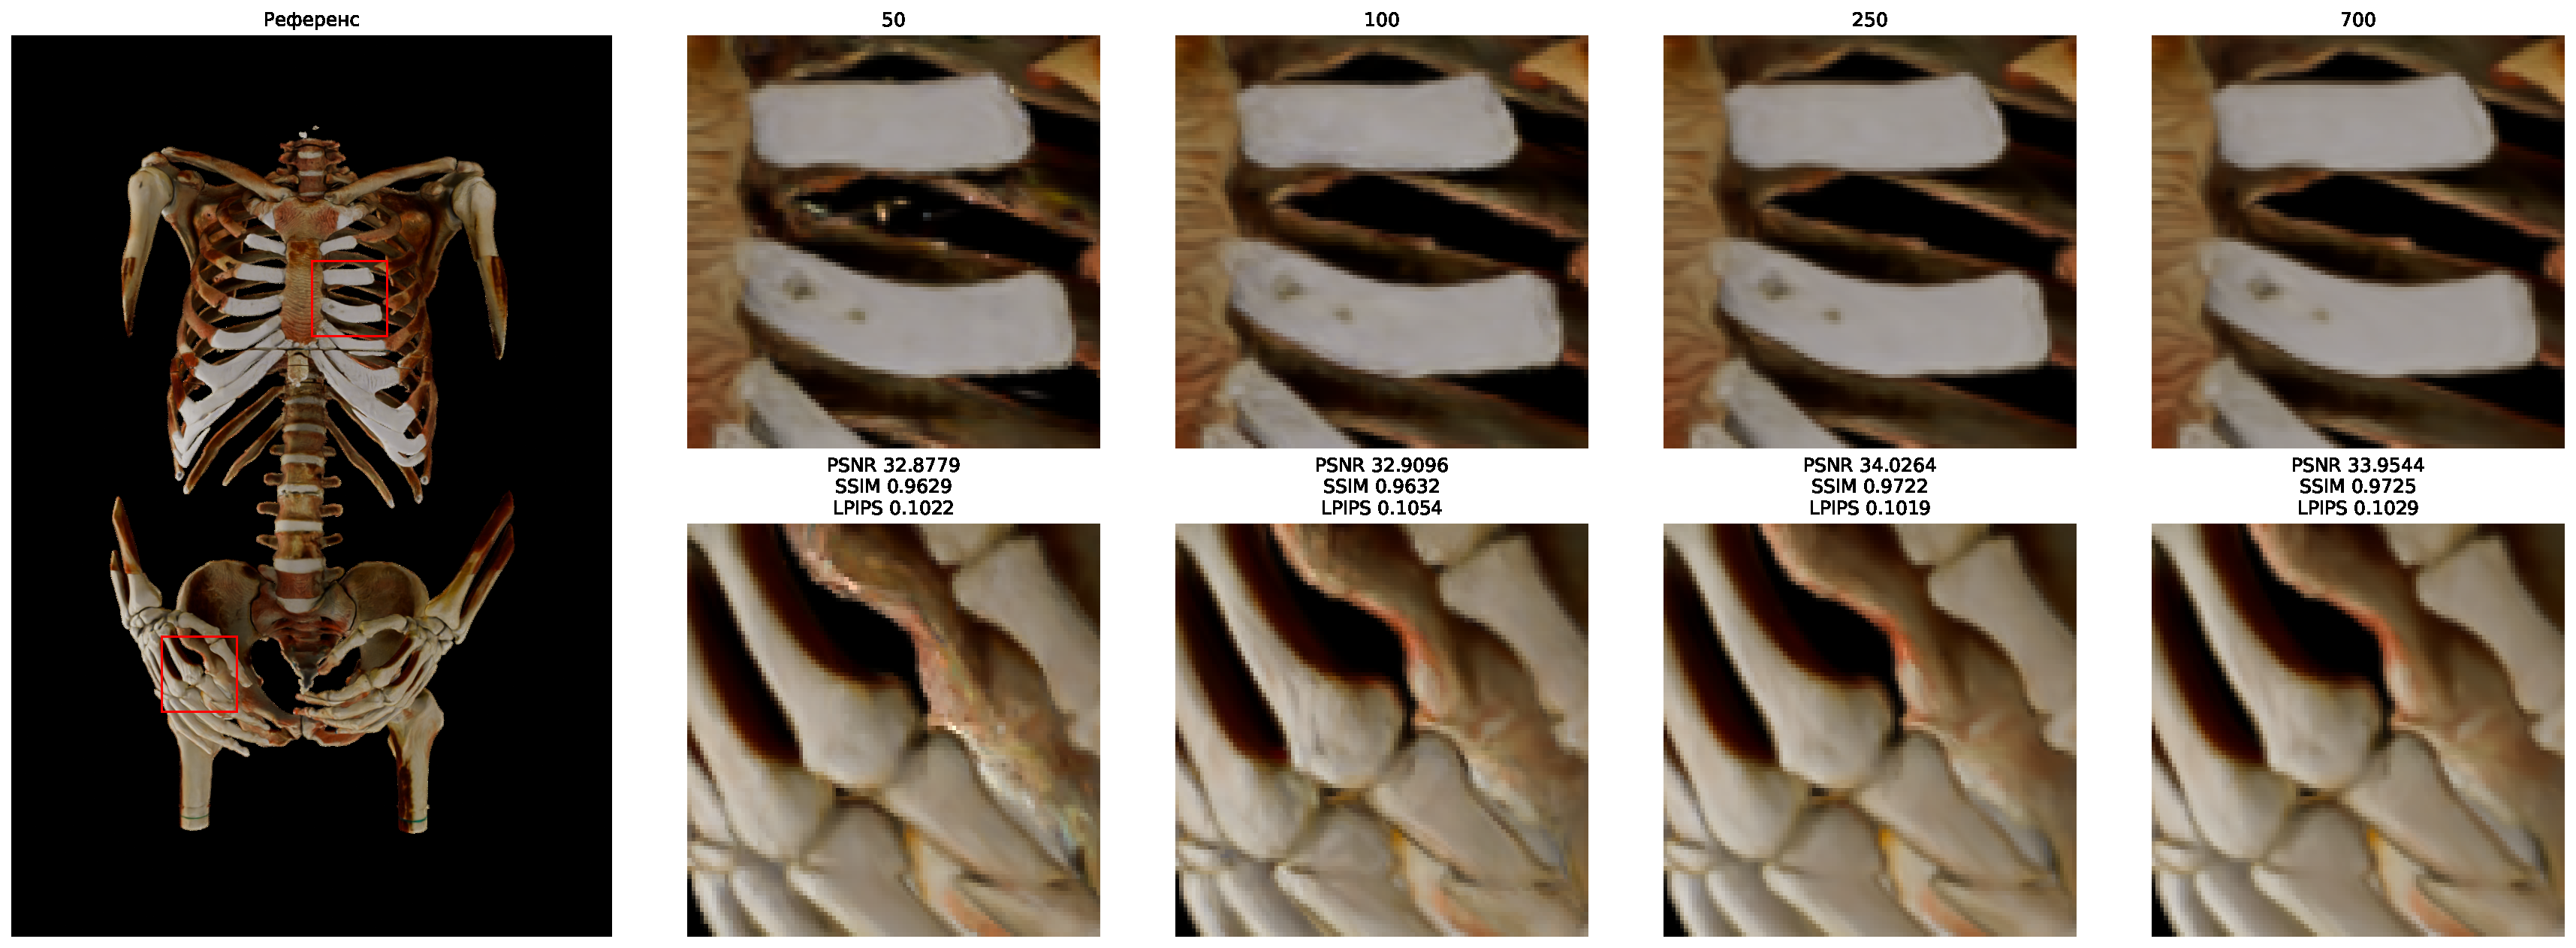
\includegraphics[width=\textwidth]{assets/50-100-250-700.pdf}
	\caption{30000 итераций различного числа референсных изображений, слева --- изображение, не участвующее в обучении; PSNR $\uparrow$, SSIM $\uparrow$, LPIPS $\downarrow$. При 50 видны артефакты, различия между 100 и 250 только по метрике, при этом между 250 и 700 не видно вообще никаких различий, в том числе по метрикам.}
	\label{fig:50-100-250-700}
\end{figure}